\documentclass{article}
\usepackage[margin=1.25in]{geometry}
\usepackage{amsmath, amssymb, setspace, enumerate, enumitem}
\usepackage{setspace}
\usepackage{graphicx}
\doublespacing

\begin{document}
    \begin{enumerate}[label=\textbf{Q1}]
        \item Give an algorithm (pseudo code, with explanation) to compute $2^{2^n}$ in linear time, assuming multiplication of arbitrary size integers takes unit time. What is the bit-complexity if multiplications do not take unit time, but are a function of the bit-length. \\
        \textbf{Solution:}\\
        Algorithm to compute $2^{2^n}$ in (close) to constant time. But yet still O(1) is a subset of O(n), therefore it falls under linear time.
        \begin{verbatim}
mult(n):
    a = 1 shifted to the left n bits
    return 1 shifted to the left a bits
        \end{verbatim}
        The bit complexity if multiplication does not take unit time would be
        $2^{2n}$, or $4^n$. As this multiplication is carried out for $n$, the
        number of bits required to represent $2^{2^n}$ will be $2^{2n}$.
    \end{enumerate}

    \begin{enumerate}[label=\textbf{Q2}]
        \item Consider the problem of computing $N! = 1 \cdot 2 \cdot 3 \cdot \cdot \cdot N$
        \begin{enumerate}[label=(\alph*)]
            \item If $N$ is an n-bit number, how many bits long is $N!$ in $O()$ notation (give the tightest bound)?\\
            \textbf{Solution:}\\
            Since $N$ is an n-bit number. We assume that $N \times N$ will be $\Theta(n^2)$ time
            complexity. However, since it is a factorial, the value multiplied will begin to get smaller.
            Since there is a decrease in the value of $N$ being multiplied, then the total running
            time for $N!$ will be $\Theta(n^2logn)$
            \item Give an algorithm to compute $N!$ and analyze its running time.\\
            \textbf{Solution:}
            \begin{verbatim}
nfactorial(n):
    int result = 0;
    for (int i = 2; i < n; i++){
        result *= i;
    }
    return result;
            \end{verbatim}
            The for loop will run $N$ times, multiplication $N \times N$ would be $n^2$ runtime,
            but since our multiplication is by an increasing value of $N$, the first numbers leading
            up to $N$ are negligeable until reaching closer to $N$. Instead of the multiplication being $\Theta(n^2)$, 
            it can be considered as $\theta(nlog n)$, We multiply $N$ times, giving
            a total time complexity of $\Theta(n^2logn)$.
        \end{enumerate}
    \end{enumerate}

    \begin{enumerate}[label=\textbf{Q3}]
        \item Find the GCD of 1492 and 1776, using
        \begin{enumerate}[label=(\alph*)]
            \item the prime factorization method and using Euclid's method, and\\
            \textbf{Prime factorization method}\\
            $1492 = 2 \times 2 \times 373$\\
            $1776 = 2 \times 2 \times 2 \times 2 \times 3 \times 37$\\
            Common factors between then are $2 \times 2$. Therefore, their gcd = $4$.\\
            \textbf{Euclid's method}\\
            gcd(1776, 1492)\\
            $1776 = 1 \times 1492 + 284$\\
            $1492 = 5 \times 284 + 72$\\
            $284 = 3 \times 72 + 68$\\
            $72 = 1 \times 68 + \underline{4}$\\
            $68 = 17 \times 4 + 0$\\
            gcd(1776, 1492) = 4
            \item express the GCD as an integer linear combination of the two inputs.\\
            \textbf{Solution: solve $\mathbf{1776x + 1492y = 4}$ for x, y}\\
            \noindent 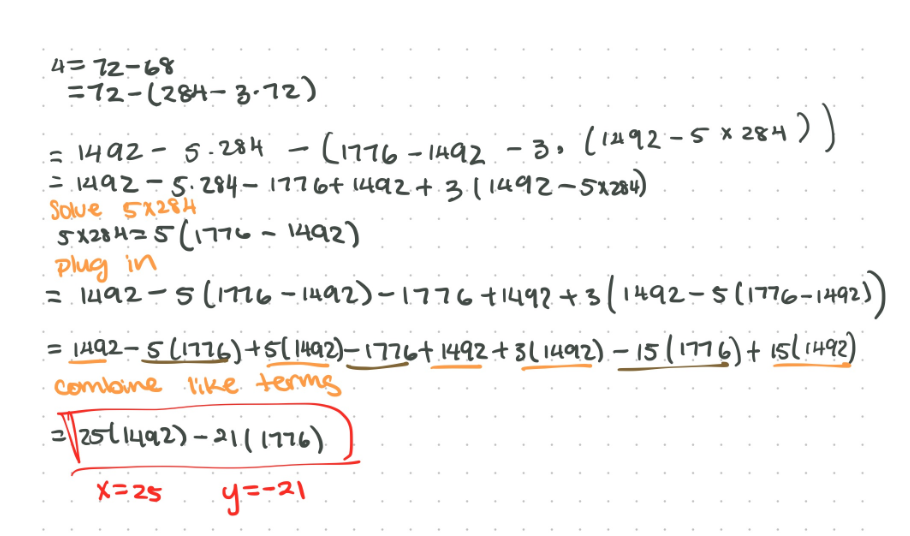
\includegraphics[scale=0.3]{problem3_b.png}
        \end{enumerate}
    \end{enumerate}
    Contributed with Jericho Dizon, Jose Idrovo, and Adrian Rodriguez
\end{document}